\documentclass{homework}
\usepackage[utf8]{inputenc}
\usepackage{amsmath}
\usepackage{amssymb}
\usepackage{braket}
\usepackage{graphicx}

% CHANGE THE FOLLOW THREE LINES!
\newcommand{\hwname}{Vaansh Lakhwara}
\newcommand{\hwemail}{ID: 401147641}
\newcommand{\hwnum}{1}

% CHANGE THESE ONLY ONCE PER CLASS
\newcommand{\hwtype}{Assignment}
\newcommand{\hwclass}{COMP 335}

\begin{document}
\maketitle

\question

\textbf{(a)}\\
\textbf{My example:}\\
L = \{(ab)$^i, 3\geq i\geq1\}$\\
\newline
\textbf{Reasoning:}\\
L = \{ab, abab, ababab\}\\
|L| = 3\\
2|L|=6
L$^R$ = \{ba, baba, bababa\}\\
L $\cup $ L$^R$ = \{ab, ba, abab, baba, ababab, bababa\}\\
|L $\cup $ L$^R$| = 6\\
$\therefore$, |L $\cup $ L$^R$| = 2|L|\\

\textbf{(b)}\\
\textbf{My example:}\\
L = \{(ab)$^i, 3\geq i\geq0\}$\\
\newline
\textbf{Reasoning:}\\
L = \{$\lambda$, ab, abab, ababab\}\\
|L| = 4\\
2|L|=8\\
L$^R$ = \{$\lambda$, ba, baba, bababa\}\\
L $\cup $ L$^R$ = \{$\lambda$, ab, ba, abab, baba, ababab, bababa\}\\
|L $\cup $ L$^R$| = 7\\
$\therefore$, |L $\cup $ L$^R$| < 2|L|\\

\textbf{(c)}\\
\textbf{Condition:}\\
I think a general condition on a non-empty finite language L that is necessary and sufficient for |L $\cup $ L$^R$| = 2|L| is for L to not have any symmetric strings in it.\\

\textbf{Reasoning:}\\
If L has a symmetric string say "aaaa",\\
then L$^R$ would also have the string "aaaa"\\
However, this would lead to their union to be less than twice the length of L\\
or, in other words |L $\cup $ L$^R$| < 2|L|\\
\\
\textbf{Example:}\\
Let L = \{ab, b, aaa, bbbb\}\\
L$^R$ = \{ba, b, aaa, bbbb\}\\
and, L $\cup $ L$^R$ = \{ab, ba\}\\
|L| = 4 \Rightarrow 2|L| = 8\\
|L $\cup $ L$^R$|= 2
$\therefore$, |L $\cup $ L$^R$| $\neq$ 2|L|\\

\question
\textbf{(a)}\\
\textbf{For M$_1$:}\\
Start state = $q_0$\\
\textbf{For M$_2$:}\\
Start state = $q_0$\\

\textbf{(b)}\\
\textbf{For M$_1$:}\\
Set of accept states = Q = \{$q_3$\}\\
\textbf{For M$_2$:}\\
Set of accept states = Q = \{$q_0$, $q_1$\}\\

\textbf{(c)}\\
\textbf{For M$_1$:}\\
Sequence of states: $q_0$, $q_0$, $q_0$, $q_1$, $q_2$, $q_2$\\
i.e, $q_0$\rightarrow$q_0$; $q_0$\rightarrow$q_0$; $q_0$\rightarrow$q_1$; $q_1$\rightarrow$q_2$; $q_2$\rightarrow$q_2$\\
\textbf{For M$_2$:}\\
Sequence of states: $q_0$, $q_1$, $q_1$, $q_2$, $q_2$, $q_2$\\
i.e, $q_0$\rightarrow$q_1$; $q_1$\rightarrow$q_1$; $q_1$\rightarrow$q_2$; $q_2$\rightarrow$q_2$; $q_2$\rightarrow$q_2$\\

\textbf{(d)}\\
\textbf{For M$_1$:}\\
No, it does not.\\
\textbf{For M$_2$:}\\
No, it does not.\\

\textbf{(e)}\\
\textbf{For both M$_1$ and M$_2$:}\\
No, they do not since it is a DFA.\\

\textbf{(f)}\\
\textbf{For M$_1$:}\\
\{(a)$^i$b(a)$^j$b(a)$^k$b(a)$^l|i,j,k,l\geq0$\}\\
\textbf{For M$_2$:}\\
\{(b$^i$a$^j$)|i,j$\geq0$\}\\
\newline
\newline
\newline
\newline
\newline
\newline
\newline
\question
\begin{center}
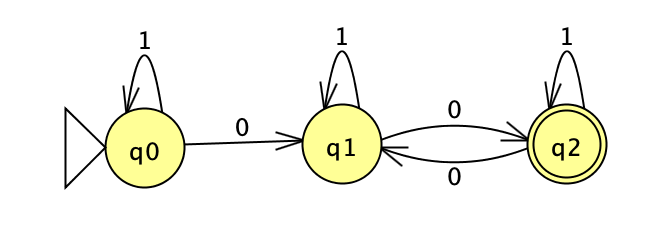
\includegraphics{A1Q3DFA1.png}\\
DFA - contains an even number of 0s\\

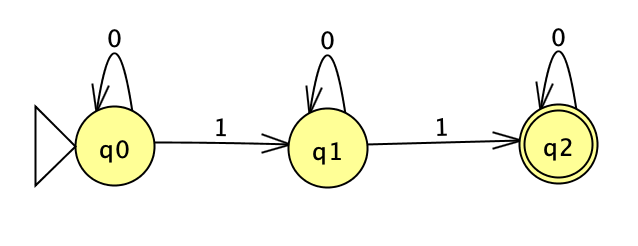
\includegraphics{A1Q3DFA2.png}\\
DFA - contains exactly two 1s\\

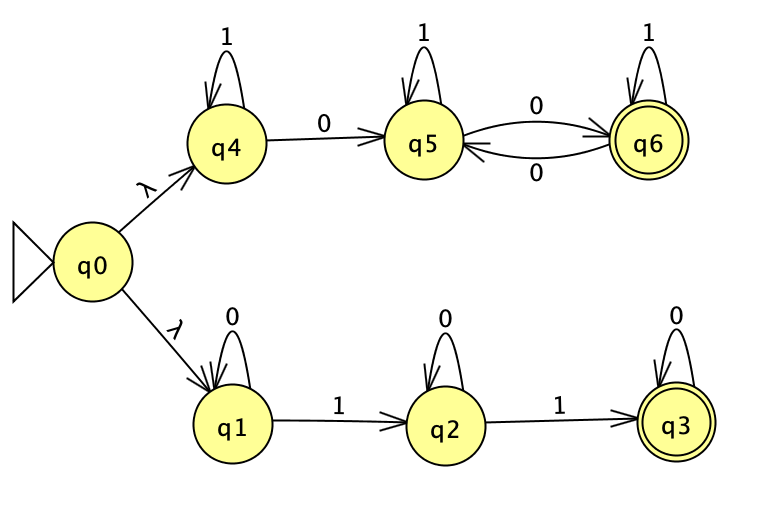
\includegraphics{A1Q3NFAFinal.png}\\
NFA by combining the two DFAs above\\
\end{center}
\begin{center}
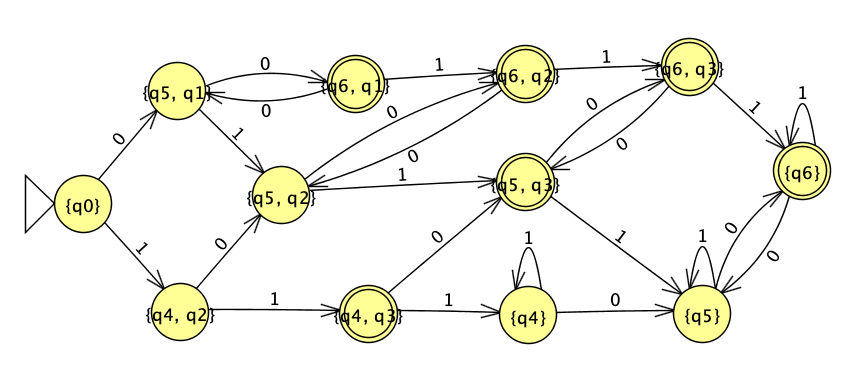
\includegraphics{A1Q3DFAFinal.png}\\
NFA converted to DFA, conversion table on the top of this page\\
\end{center}
\begin{center}
\begin{table}[]
\begin{tabular}{|l|l|l|}
\hline
           & 0          & 1          \\ \hline
\{q0\}     & \{q5, q1\} & \{q4, q2\} \\ \hline
\{q5, q1\} & \{q6, q1\} & \{q5, q2\} \\ \hline
\{q4, q2\} & \{q5, q2\} & \{q4, q3\} \\ \hline
\{q6, q1\} & \{q5, q1\} & \{q6, q2\} \\ \hline
\{q5, q2\} & \{q6, q2\} & \{q5, q3\} \\ \hline
\{q4, q3\} & \{q5, q3\} & \{q4\}     \\ \hline
\{q6, q2\} & \{q5, q2\} & \{q6, q3\} \\ \hline
\{q5, q3\} & \{q6, q3\} & \{q5\}     \\ \hline
\{q4\}     & \{q5\}     & \{q4\}     \\ \hline
\{q6, q3\} & \{q5, q3\} & \{q6\}     \\ \hline
\{q5\}     & \{q6\}     & \{q5\}     \\ \hline
\{q6\}     & \{q5\}     & \{q6\}     \\ \hline
\end{tabular}
\end{table}
A simplified version of this diagram would be:\\
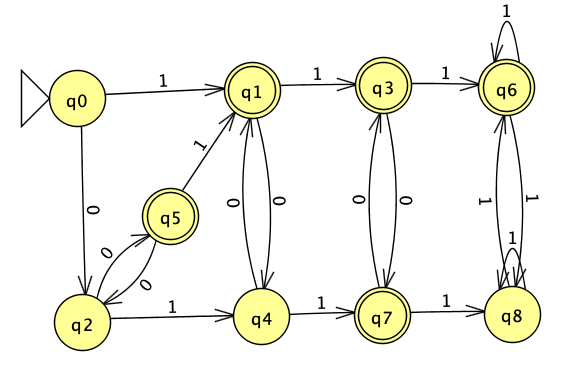
\includegraphics{A1Q3DFAFinal1.png}\\
\end{center}
\end{document}